\chapter{Введение}

\begin{figure}[H]
    \centering
    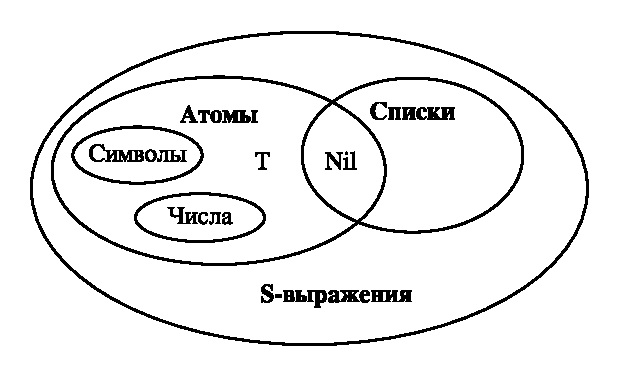
\includegraphics{img/expression.pdf}
\end{figure}

\section{Классификация функций}

\begin{enumerate}
    \item \textbf{Чистые математические функцие}
        (фиксированное количество аргументов, всегда возращает
        один результат)
    \item \textbf{Форма}
        (функции, которые имеют переменное количество аргументов либо
        они по-разному обрабатывают все аргументы)
    \item \textbf{Функцианал}
        (вместо одного из аргументов принимает функцию)
\end{enumerate}

\section{Базис языка}

\textbf{Базис языка} -- базовые структуры и атомы и базовые функции.

\subsection{Классификация базисных функций}

\begin{itemize}
    \item \textbf{Функции селекторы}

        \begin{itemize}
            \item {\ttfamily car}
            \item {\ttfamily cdr}
        \end{itemize}

    \item \textbf{Работа со списками}

        \begin{itemize}
            \item Создание списка --
                {\ttfamily cons} (два указателя)

                {\ttfamily (cons 'A 'B)} -- точечная пара

                {\ttfamily (cons 'A '(B))} -- список

            \item Создание списковых ячеек по количеству агрументов --
                {\ttfamily list} (произволтное количество агрументов)

                {\ttfamily (list 'A 'B)} -- список
        \end{itemize}

    \item \textbf{Предикаты}

        Все что не {\ttfamily Nil}, то {\ttfamily T (True)}

        \begin{itemize}
            \item Атом или нет -- {\ttfamily atom}
            \item Пустой список или нет -- {\ttfamily Null}
            \item Список или нет (или списковые ячейки) --
                {\ttfamily consp}
        \end{itemize}

    \item \textbf{Функции сравнения объектов}

        \begin{itemize}
            \item {\ttfamily eq} -- сравнивает по указателю
            \item {\ttfamily eql} -- сравнивает числа одного типа
                (синтаксической формы представления)

                {\ttfamily (eql 3 3.0) -- Nil}

                {\ttfamily (eql 3 3) -- T}

            \item {\ttfamily =} -- сравнивает числа по значению

                {\ttfamily (= 3 3.0) -- T}

            \item {\ttfamily equal} -- корректно сравнивает списки
            \item {\ttfamily equalp} -- наиболее качественно и долго
        \end{itemize}
\end{itemize}

\subsection{Способы определения функций}

\subsubsection{С именем}

\begin{lstlisting}
( defun fn(args)
    (S-expression)
)
\end{lstlisting}

\subsubsection{Без имени}

\begin{lstlisting}
(lambda (args)
    (S-expression)
)
\end{lstlisting}

\begin{lstlisting}
(apply #'($\lambda$ expression) arg1...argN)
\end{lstlisting}

\begin{lstlisting}
(fncall #'($\lambda$ expression) arg1...argN)
\end{lstlisting}

\subsection{Атом в памяти}

\begin{figure}[H]
    \centering
    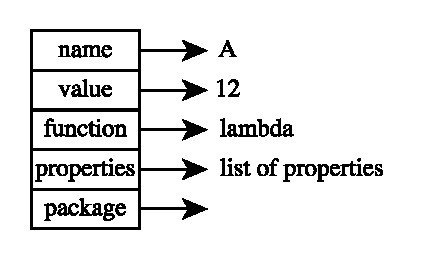
\includegraphics[scale=1.5]{img/atom.pdf}
\end{figure}

\subsubsection{Установка значения в атом}

\begin{lstlisting}
(setq 'A 12)
\end{lstlisting}

\subsection{Диаграмма вычисления S-выражения}

\begin{figure}[H]
    \centering
    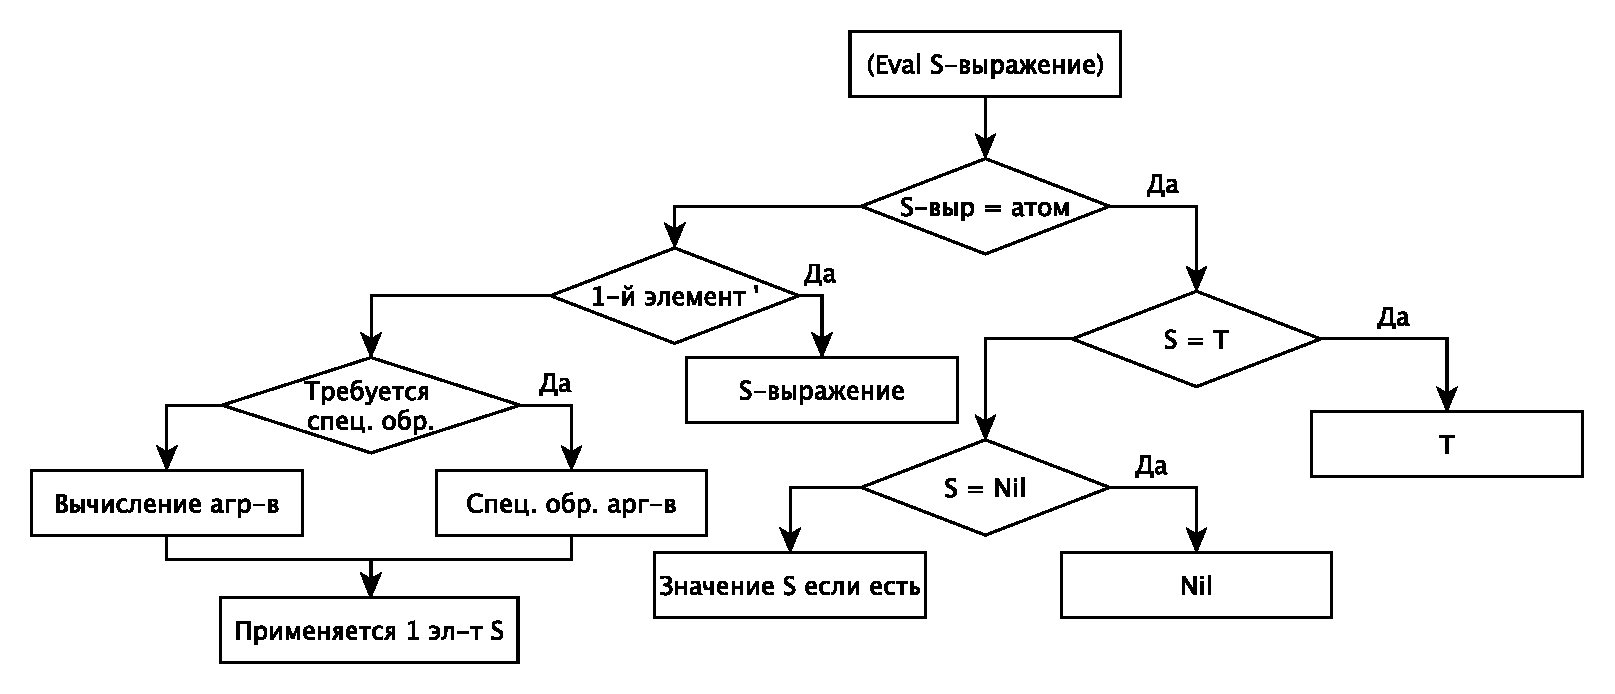
\includegraphics[scale=0.7]{img/running.pdf}
\end{figure}

\section{Специальные формы}

\subsection{Ветвление}

\begin{lstlisting}
(cond ((conditional1) (body1))
      ((conditional2) (body2))
)
\end{lstlisting}

\subsection{Условный оператор}

\begin{lstlisting}
(if (conditional) (t-body) (f-body))
\end{lstlisting}

\subsection{Локальные переменные}

\begin{lstlisting}
(let
    (var1 value1)
    (var2 value2)
    ...
    (varN valueN)
    body
)
\end{lstlisting}

Сначала вычисляются все значения {\ttfamily value}, и только потом
они связываются с переменными, поэтому сослаться на переменную
до тела нельзя.

\begin{lstlisting}
(let*
    (var1 value1)
    (var2 value2)
    ...
    (varN valueN)
    body
)
\end{lstlisting}

Здесь уже можно обращаться до тела.

\section{Функции модификации списков}

\begin{itemize}
    \item Структуроразрушающие
    \item Не разрушающие структуру
\end{itemize}

\begin{enumerate}
    \item {\ttfamily (append list1 list2)}
        Работает с копиями, создаются копии всех элементов
    \item {\ttfamily (reverse list)} --
    \item {\ttfamily (nreverse list)}
    \item {\ttfamily nconc} --
        конкатенация
    \item {\ttfamily last} --
        последний элемент
    \item {\ttfamily (nth n list)} --
        n-я списковая ячейка (нумерация с 0)
    \item {\ttfamily (nthcdr n list)} --
        хвост n-списковой ячейки
    \item {\ttfamily (length list)} --
        количество списковых ячеек на верхнем уровне
    \item {\ttfamily (remove el list)} --
        удаление элемента (сравнение с помощью {\ttfamily eql})
    \item {\ttfamily (rplaca list el)}
    \item {\ttfamily (rplacd list el)}
    \item {\ttfamily (member el list)} --
        проверяет есть ли элемент среди списковых ячеек верхнего уровня
        (возвращает список, начинающийся с перврого вхождения элемента)
        используется {\ttfamily eql}, которая не сравнивает списки
    \item {\ttfamily (union list1 list2)} --
        множество из двух список (без дубликатов)
    \item {\ttfamily (intersection list1 list2)} --
        пересечение множеств
    \item {\ttfamily (set\_difference list1 list2)} --
        разность множеств
    \item {\ttfamily (assoc key list)} --
        работает с ассоциативной таблицей
        (возвращается списковая ячейка, где ключ совпадает с искомым)
    \item {\ttfamily (rassoc value list)} --
        работает с ассоциативной таблицей
        (возвращается списковая ячейка,
        где значение совпадает с искомым)
    \item {\ttfamily (acons)} --
        добавление нового элемента в ассоциативный список
\end{enumerate}

\section{Ключевые параметры}

\begin{lstlisting}
(member '(a b) (f (a b) c) : test #'equal)
\end{lstlisting}

Вместо стандартного {\ttfamily eql} будет использоваться
{\ttfamily equal}.

\section{Функционалы}

\begin{enumerate}
    \item {\ttfamily (mapcar \#'fun list)}
    \item {\ttfamily (mapcar \#'fun list1 list2 ... listN)}
    \item {\ttfamily (maplist \#'fun list)}
    \item {\ttfamily (mapcan)} --
        разрушают структуру (работает эффективней)
    \item {\ttfamily (reduce #'+ '(1 2 3))} --
        применяет функцию каскадным образом
\end{enumerate}

В качестве функций могут выступать предикаты
